\section{Gestione runtime dei componenti, il meccanismo change detection}
Per consentire l'aggiornamento runtime  del DOM a seguito delle modifiche delle proprietà dei componenti, Angular sfrutta un meccanismo chiamato change detection.
\newline
 La libreria costruisce un albero composto dai componenti renderizzati e, quando viene lanciato il meccanismo di change detection, essa esegue una visita top down dell'albero in cerca dei componenti le quali proprietà sono state modificate e ne renderizza di nuovo la view. Angular esegue questa operazione solo per le proprietà che vengono utilizzate nel template e per ognuna esegue un controllo con il valore precedente.
\newline
\begin{figure}[H]
\centering
   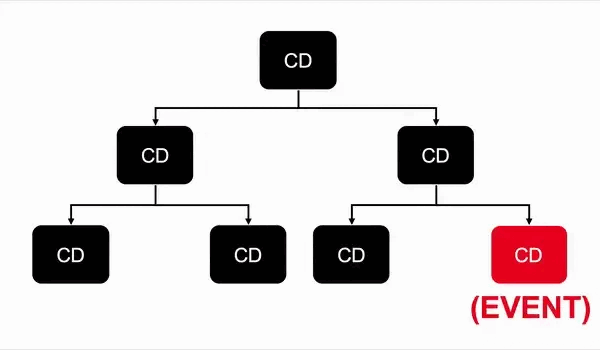
\includegraphics[scale=0.5]{resources/cd-1.png}
\caption{un componente viene modificato e lancia il meccanismo di change detection}
\end{figure}
\begin{figure}[H]
\centering
   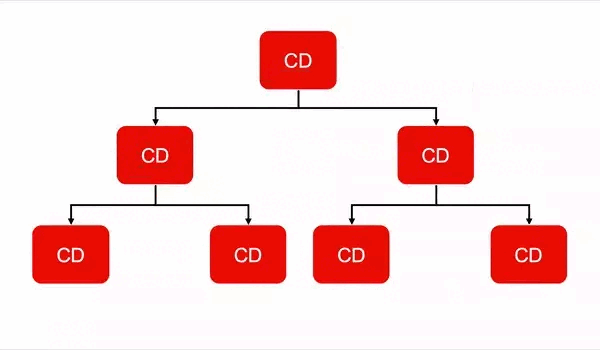
\includegraphics[scale=0.5]{resources/cd-2.png}
\caption{l'albero viene visitato alla ricerca di proprietà modificate}
\end{figure}





